\section{Sensitivity analysis}

We now consider further developments arising from the notion of duality in linear programming problems. We begin by focusing on the employment of the dual simplex method and the interpretation of the dual multipliers, as discussed in Chapter \ref{chapter_5}. 

Specifically, assume that we have solved to optimality the problem $P$ given as
%
\begin{align*}
	P : \mini \, &c^\top x \\
	\st \, & Ax = b \\
	& x \geq 0. 	
\end{align*}
%
As we have seen in Chapter \ref{chapter_4}, the optimal solution $\overline{x}$ with associated basis $B$ satisfies the following optimality conditions: it is a \emph{basic feasible solution} and, therefore (i) $B^{-1}b \geq 0$; and (ii) all reduced costs are nonnegative, that is $c^\top - c_B^\top B^{-1}b \geq 0$.

We are interested in analysing aspects associated with the \emph{stability} of the optimal solution $\overline{x}$ in terms of how it changes with the inclusion of new decision variables and constraints or in with changes in the input data. Both cases are somewhat motivated by the realisation that problems typically emerge from dynamic settings. Thus, one must assess how \emph{stable} a given plan (represented by $\overline{x}$) is or how it can be adapted in face of changes in the original problem setting. This kind of analysis is generally referred to as \emph{sensitivity analysis} in the context of linear programming.

First, we will consider the inclusion of new variables or new constraints \emph{after} the optimal solution $\overline{x}$ is obtained. This setting represents, for example, the inclusion of a new product or a new production plant (referring to the context of resource allocation and transportation problems, as discussed in Chapter \ref{chapter_1}) or the consideration of additional constraints imposing new (or previously disregarded) requirements or conditions. The techniques we will consider here will also be relevant in the following chapters. We will then discuss specialised methods for large-scale problems and solution techniques for integer programming problems, both topics that heavily rely on the idea of iteratively incrementing linear programming problems with additional constraints (or variables).

The second group of cases relates to changes in the input data. When utilising linear programming models to optimise systems performance, one must bear in mind that there is inherent uncertainty associated with the input data. Be it due to measurement errors or a lack of complete knowledge about the future, one must accept that the input data of these models will, by definition, embed some measure of error. One way of taking this into account is to try to understand the consequences to the optimality of $\overline{x}$ in case of eventual changes in the input data, represented by the matrix $A$, and the vectors $c$ and $b$. We will achieve this by studying the ranges within which variations in these terms do not compromise the optimality of $\overline{x}$. 


\subsection{Adding a new variable} \label{section_611}

Let us consider that a new variable $x_{n+1}$ with associated column (that is, respective objective function and constraint coefficients) $(c_{n+1}, A_{n+1})$ is added to $P$. This leads to a new augmented problem $P'$ of the form
%
\begin{align*}
	P': \mini \, &c^\top x + c_{n+1}x_{n+1}\\
	\st \, & Ax + A_{n+1}x_{n+1}= b \\
	& x \geq 0, x_{n+1} \geq 0. 	
\end{align*}
%
We need to determine if, after the inclusion of this new variable, the current basis $B$ is still optimal. If we make the newly added variable nonbasic yields the basic feasible solution (BFS) $x = (\overline{x}, 0)$. Moreover, we know that the optimality condition $c^\top - c_B^\top B^{-1}b \geq 0$ held before the inclusion of the variable, so we know that all the other reduced costs associated with the nonbasic variables $j \in I_N$ were nonnegative. 

Therefore, the only check that needs to be done is whether the reduced cost associated with $x_{n+1}$ also satisfies the optimality condition, i.e., if
%
\begin{equation*}
	\overline{c}_{n+1} = c_{n+1} - c_B^\top B^{-1}A_{n+1} \geq 0.	
\end{equation*}
%
If the optimality condition is satisfied, the new variable does not change the optimal basis, and the solution $x = (\overline{x}, 0)$ is optimal. Otherwise, one must perform a new simplex iteration, using $B$ as a starting BFS. Notice that in this case, primal feasibility is trivially satisfied, while dual feasibility is not observed (that is, $\overline{c}_{n+1} < 0$). Therefore, primal simplex can be employed, \emph{warm started} by $B$. This is often a far more efficient strategy than resolving $P'$ from scratch.


%TODO: Chp6: Change this to the paint example
Let us consider a numerical example. Consider the problem
%
\begin{align*}
	\mini & -5x_1 -x_2 + 12 x_3 \\
	\st   & 3x_1 + 2x_2 + x_3 = 10 \\
	& 5x_1 + 3x_2 + x_4 = 16 \\
	& x_1, \dots, x_4 \geq 0.
\end{align*}
%
The tableau associated with its optimal solution is given by

\begin{center}
	\begin{tabular}{r|cccc|c} 
	   &$x_1$ & $x_2$ & $x_3$ & $x_4$& RHS \\ \hline	
	   $z$ & 0 & 0 & 2 & 7 & 12\\ \hline
	   $x_1$ & 1 & 0 & -3 & 2 & 2\\
	   $x_2$ & 0 & 1 & 5 & -3 & 2            
	\end{tabular}
\end{center}

Suppose we include a variable $x_5$, for which $c_5 = -1$ and $A_5 = (1,1)$. The modified problem then becomes
%
\begin{align*}
	\mini & -5x_1 -x_2 + 12 x_3 -x_5 	 \\
	\st   & 3x_1 + 2x_2 + x_3 + x_5 = 10 \\
	& 5x_1 + 3x_2 + x_4 + x_5 = 16 \\
	& x_1, \dots, x_5 \geq 0.
\end{align*}
%
We have that the reduced cost of the new variable is given by $\overline{c}_5 = c_5 - c_B^\top B^{-1}A_5 = -4$ and $B^{-1}A_5 = (-1,2)$. The tableau for the optimal basis $B$ considering the new column associated with $x_5$ is thus

\begin{center}
	\begin{tabular}{r|ccccc|c} 
	   &$x_1$ & $x_2$ & $x_3$ & $x_4$& $x_5$ & RHS \\ \hline	
	   $z$ & 0 & 0 & 2 & 7 & -4 & 12   \\ \hline
	   $x_1$ & 1 & 0 & -3 & 2 & -1 & 2 \\
	   $x_2$ & 0 & 1 & 5 & -3 & 2 & 2	            
	\end{tabular}
\end{center}

Notice that this tableau now shows a primal feasible solution that is not optimal and can be further iterated using primal simplex.


\subsection{Adding a new constraint} \label{section_612}

We now focus on the inclusion of additional constraints. Let us assume that a general constraint of the form ${a_{m+1}}^\top x \geq b_{m+1}$ is added to $P$. We assume it to be an inequality that has been applied to problem $P$, which was originally in the standard form, after it was solved.

The first thing to notice is that, if the optimal solution $\overline{x}$ to $P$ satisfy ${a_{m+1}}^\top \overline{x} \geq b_{m+1}$, then nothing changes. Otherwise, we need to rewrite the new constraint accordingly by including a slack variable, obtaining 
%
\begin{equation*}
	{a_{m+1}}^\top x - x_{n+1} = b_{m+1}.
\end{equation*}
%
Notice that doing so changes the matrix $A$ of the original problem $P$, which becomes
%
\begin{equation*}
	\overline{A} = \begin{bmatrix}
				   A & 0 \\ a^\top_{m+1} & -1 
				   \end{bmatrix}.
\end{equation*}

We can reuse the optimal basis $B$ to form a new basis $\overline{B}$ for the problem. This will have the form
%
\begin{equation*}
	\overline{B} = \begin{bmatrix}
		B & 0 \\ a^\top & -1 
	\end{bmatrix},	
\end{equation*}
%
where $a$ are the respective components of $a_{m+1}$ associated with the columns from $A$ that formed $B$. Now, since we have that $\overline{B}^{-1}\overline{B} = I$, we must have that 
%
\begin{equation*}
	\overline{B}^{-1} = \begin{bmatrix}
		B^{-1} & 0 \\ a^\top B^{-1} & -1 
	\end{bmatrix}.	
\end{equation*}
%
Notice however, that the basic solution $(\overline{x}, {a_{m+1}}^\top \overline{x} -  b_{m+1})$ associated with $\overline{B}$ is not feasible, since we assumed that $\overline{x}$ did not satisfy the newly added constraint, i.e., ${a_{m+1}}^\top \overline{x} < b_{m+1}$.

The reduced costs considering the new basis $\overline{B}$ then becomes
%
\begin{equation*}
	[c^\top ~~ 0] - [c_B^\top ~~ 0]\begin{bmatrix} B^{-1} & 0 \\ a^\top B^{-1} & -1 \end{bmatrix}\begin{bmatrix} A & 0 \\ a_{m+1}^\top & -1 \end{bmatrix} = [c^\top - c^\top_B B^{-1}A ~~ 0].
\end{equation*}
  	
Notice that the new slack variable has a null component as a reduced cost, meaning that it does not violated dual feasibility conditions. Thus, after adding a constraint that makes $\overline{x}$ infeasible, we still have a dual feasible solution that can be immediately used by the dual simplex method, again allowing for warm starting the solution of the new problem.

To build an initial solution in terms of the tableau representation of the simplex method, we must simply add an additional row, which leads to a new tableau with the following structure
%
\begin{equation*}
	\overline{B}^{-1}A = \begin{bmatrix} B^{-1}A & 0 \\ a^\top B^{-1}A - a_{m+1}^\top & 1 \end{bmatrix}.
\end{equation*}
%		

Let us consider a numerical example again. Consider the same problem as the previous example, but that we instead include the additional constraint $x_1 + x_2 \geq 5$, which is violated by the optimal solution $(2,2,0,0)$. In this case, we have that $a_{m+1} = (1,1,0,0)$ and $a^\top B^{-1} A - a^\top_{m+1} = [0, 0, 2, -1]$. This modified problem then looks like
%
%TODO: Chp6: Change this to the paint example
\begin{align*}
	\mini & -5x_1 -x_2 + 12 x_3 \\
	\st   & 3x_1 + 2x_2 + x_3  = 10 \\
	& 5x_1 + 3x_2 + x_4 = 16 \\
	& -x_1 - x_2 + x_5 = -5  \\
	& x_1, \dots, x_5 \geq 0
\end{align*}
%
with associated tableau

\begin{center}
	\begin{tabular}{r|ccccc|c} 
	   &$x_1$ & $x_2$ & $x_3$ & $x_4$ & $x_5$ & RHS \\ \hline	
	   $z$ & 0 & 0 & 2 & 7 & 0 & 12                 \\ \hline
	   $x_1$ & 1 & 0 & -3 & 2 & 0 & 2 				\\
	   $x_2$ & 0 & 1 & 5 & -3 & 0 & 2 				\\
	   $x_5$ &  0 &  0 &  2 & -1 & 1 & -1           
	\end{tabular}
\end{center}

Notice that this tableau indicates that we have a dual feasible solution that is not primal feasible and thus suitable to be solved using dual simplex.
	
A final point to note is that these operations are related to each other in terms of equivalent primal-dual formulations. That is, consider dual of $P$, which is given by
%
\begin{align*}
	D : \maxi   & p^\top b \\
	\st 			& p^\top A \le c.
\end{align*}
%
Then, adding a constraint of the form $p^\top A_{n+1} \leq c_{n+1}$ is equivalent to adding a variable to $P$, exactly as discussed in Section \ref{section_611}.


\subsection{Changing input data} \label{section_613}

We now consider how changes in the input data can influence the optimality of a given basis. Specifically, we consider how to predict whether changes in the vector of independent terms $b$ and objective coefficients $c$ will affect the optimality of the problem. Notice that variations in the coefficient matrix $A$ are left aside.

%TODO: Chp6: include a discussion on variations on the coefficients of A.

\subsubsection{Changes in the vector $b$}

Suppose that some component $b_i$ changes and becomes $b_i + \delta$, with $\delta \in \reals$. We are interested in the range for $\delta$ within which the basis $B$ remains optimal.

First, we must notice that optimality conditions $\overline{c} = c^\top - c^\top_B B^{-1}A \geq 0$ are not directly affected by variation in the vector $b$. This means that the choice of variable indices $j \in I_B$ to form the basis $B$ will, in principle, be \emph{stable} unless the change in $b_i$ is such that $B$ is rendered \emph{infeasible}. Thus, we need to study the conditions in which  feasibility is retained, or, more specifically, if (recall the $e_i$ is the vector of zeros except for the $i\nth$ component being 1)
%
\begin{equation*}
	B^{-1}(b + \delta e_i) \geq 0.	
\end{equation*}

Let $g = (g_{1i}, \dots, g_{mi})$ be the $i\nth$ column of $B^{-1}$. Thus
%
\begin{equation*}
	B^{-1}(b + \delta e_i) \geq 0 \Rightarrow x_B + \delta g \geq 0 \Rightarrow x_{B(j)} + \delta g_{ji} \geq 0, j = 1,\dots, m.  
\end{equation*}
%
Notice that this is equivalent to having $\delta$ within the range
%
\begin{equation*}
	\max_{j : g_{ji} > 0}\left(-\frac{x_{B(j)}}{g_{ji}}\right) \leq \delta \leq \min_{j : g_{ji} < 0}\left(-\frac{x_{B(j)}}{g_{ji}}\right).	
\end{equation*}

In other words, changing $b_i$ will incur changes in the value of the basic variables, and thus, we must determine the range within which all basic variables remain nonnegative (i.e., feasible).

Let us consider a numerical example. Once again, consider the problem from Section \ref{section_611}. The optimal tableau was given by
%TODO: Chp6: Change this to the paint example

\begin{center}
	\begin{tabular}{c|cccc|c} 
	   &$x_1$ & $x_2$ & $x_3$ & $x_4$& RHS \\ \hline	
	   $z$ & 0 & 0 & 2 & 7 & 12\\
	   $x_1$ & 1 & 0 & -3 & 2 & 2\\
	   $x_2$ & 0 & 1 & 5 & -3 & 2\\	            
	\end{tabular}	
\end{center}

Suppose that $b_1$ will change by $\delta$ in the constraint $3x_1 + 2x_2 + x_3  = 10$. Notice that the first column of $B^{-1}$ can be directly extracted from the optimal tableau and is given by $(-3,5)$. The optimal basis will remain feasible if $2 - 3\delta \geq 0$ and $2 + 5\delta \geq 0$, and thus $-2/5 \leq \delta \leq 2/3$.

Notice that this means that we can calculate the change in the objective function value as a function of $\delta \in [-2/5, 2/3]$. Within this range, the optimal cost changes as 
%
\begin{equation*}
	c_B^\top (b + \delta e_i) = p^\top b + \delta p_i,	
\end{equation*}
%
where $p^\top = c_B ^\top B^{-1}$ is the optimal dual solution. In case the variation falls outside that range, this means that some of the basic variables will become negative. However, since the dual feasibility conditions are not affected by changes in $b_i$, one can still reutilise the basis $B$ using dual simplex to find a new optimal solution.


\subsubsection{Changes in the vector $c$}

We now consider the case where variations are expected in the objective function coefficients. Suppose that some component $c_j$ becomes $c_j + \delta$. In this case, optimality conditions become a concern. Two scenarios can occur. First, it might be that the changing coefficient is associated with a variable $j \in J$ that happens to be nonbasic ($j \in I_N$) in the optimal solution. In this case, we have that optimality will be retained as long as the nonbasic variable remains ``not attractive'', i.e., the reduced cost associated with $j$ remains nonnegative. More precisely put, the basis $B$ will remain optimal if
%
\begin{equation*}
	(c_j + \delta) - c_BB^{-1}A_j \geq 0 \Rightarrow \delta \geq -\overline{c}_j.
\end{equation*}
%

The second scenario concerns changes in variables that are basic in the optimal solution, i.e., $j \in I_B$. In that case, the optimality conditions are directly affected, meaning that we have to analyse the range of variation for $\delta$ within which the optimality conditions are maintained, i.e., the reduced costs remain nonnegative.

Let $c_j$ is the coefficient of the $l^{\text{th}}$ basic variable, that is $j = B(l)$. In this case, $c_B$ becomes $c_B + \delta e_l$, meaning that all optimality conditions are simultaneously affected. Thus, we have to define a range for $\delta$ in which the condition
%
\begin{equation*}
	(c_B + \delta e_i)^\top B^{-1}A_i \leq c_i, \, \forall i \neq j 
\end{equation*}
%
holds. Notice that we do not need to consider $j$ since $x_j$ is a basic variable, and thus, its reduced costs are assumed to remain zero.

Considering the tableau representation, we can use the $l^{\text{th}}$ row and examine the conditions for which $\delta q_{li} \leq \overline{c}_i, \forall i \neq j$, where $q_{li}$ is the $l^{\text{th}}$ entry of $B^{-1}A_i$.

Let us once again consider the previous example, with optimal tableau 

\begin{center}
	\begin{tabular}{c|cccc|c} 
	   &$x_1$ & $x_2$ & $x_3$ & $x_4$& RHS \\ \hline	
	   $z$ & 0 & 0 & 2 & 7 & 12\\
	   $x_1$ & 1 & 0 & -3 & 2 & 2\\
	   $x_2$ & 0 & 1 & 5 & -3 & 2\\	            
	\end{tabular}	
\end{center}

First, let us consider variations in the objective function coefficients of variables $x_3$ and $x_4$. Since both variables are nonbasic in the optimal basis, the allowed variation for them is given by
%
\begin{equation*}
	\delta_3 \geq -\overline{c}_3 = -2 \text{ and } 
    \delta_4 \geq -\overline{c}_4 = -7. 	
\end{equation*}
%
Two points to notice. First, notice that both intervals are one-sided. This means that one should only be concerned with variations that decrease the reduced cost value, since increases in their value can never cause any changes in the optimality conditions. Second, notice that the allowed variation is trivially the negative value of the reduced cost. For variations that turn the reduced costs negative, the current basis can be utilised as a starting point for the primal simplex.

Now, let us consider a variation in the basic variable $x_1$. Notice that in this case we have to analyse the impact in all reduced costs, with exception of $x_1$ itself. Using the tableau, we have that $q_l = [1, 0, -3, 2]$ and thus
%
\begin{align*}
	& \delta_1 q_{12} \leq \overline{c}_2 \Rightarrow 0 \leq 0 \\
	& \delta_1 q_{13} \leq \overline{c}_3 \Rightarrow \delta_1 \geq -2/3  \\
	& \delta_1 q_{14} \leq \overline{c}_4 \Rightarrow \delta_1 \leq 7/2, 
\end{align*}
%
implying that $-2/3 \leq \delta_1 \leq 7/2$. Like before, for a change outside this range, primal simplex can be readily employed.


\section{Cones and extreme rays}

We now change the course of our discussion towards some results that will be useful in identifying two non-ordinary situations when employing the simplex method: unboundedness and infeasibility. Typically, these are consequences of issues related to the data and/or with modelling assumptions and are challenging in that they prevent us from obtaining a solution from the model. As we will see, they also rely on duality in their derivations and are all connected by the notion of cones, which we formally give in Definition \ref{p1c6:def:cone}.

\begin{definition}[Cones]\label{p1c6:def:cone}
	A set $C \subset \reals^n$ is a cone if $\lambda x \in C$ for all $\lambda \geq 0$ and all $x \in C$.	
\end{definition}

A cone $C$ can be understood as a set formed by the nonnegative scaling  of a collection of vectors $x \in C$. Notice that it implies that $ 0 \in C$. Often, it will be the case that $ 0 \in C$ is an extreme point of $C$ and in that case, we say that $C$ is \emph{pointed}. As one might suspect, in the context of linear programming, we will be mostly interested in a specific type of cone, those known are \emph{polyhedral cones}. Polyhedral cones are sets of the form 
%
\begin{equation*}
	P = \braces{x \in \reals^n : Ax \geq 0}.
\end{equation*}
%
Figure \ref{p1c6:fig:poly_cone} illustrates a polyhedral cone in $\reals^3$ formed by the intersection of three half-spaces. 
%
\begin{figure}[h]
	\begin{tikzpicture}
		\node (pic) at (0,0) {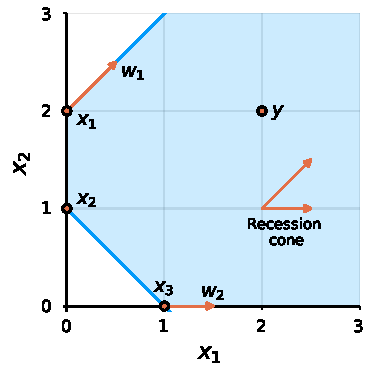
\includegraphics{part_1/chapter_6/figures/Figure1.pdf}};
		\node (x1) at (2,-2) {$x_1$};
		\node (x2) at (2,-1) {$x_2$};
		\node[right] (x3) at (-2,2) {$x_3$};
		\node (a1) at (-0.3,0.8) {$a_1$};
		\node (a2) at (1.1,-0.4) {$a_2$};
	\end{tikzpicture}
	\caption{A polyhedral cone in $\reals^3$ formed by 3 half-space} \label{p1c6:fig:poly_cone}
\end{figure}
%

Some interesting properties can be immediately concluded regarding polyhedral cones. First, they are convex sets, since they are polyhedral sets (cf. Theorem \ref{p1c2:thm:convexity}). Also, the origin is an extreme point, and thus, polyhedral cones are always pointed. Furthermore, just like general polyhedral sets, a cone $C \in \reals^n$ will always be associated with a collection of $n$ linearly independent vectors. Corollary \ref{p1c6:cor:polyhedral_cones} summarises these points. Notice we pose it as a Corollary because these are immediate consequences of Theorem \ref{p1c3:thm:exist_extreme_point}. 

\begin{corollary}\label{p1c6:cor:polyhedral_cones} 
	Let $C \subset \reals^n$ be a polyhedral cone defined by constraints $\braces{a_i^\top x \geq 0}_{i =1,\dots,m}$. Then the following are equivalent
	\begin{enumerate}
		\item $0$ is an extreme point of $C$;
		\item $C$ does not contain a line;
		\item There exists $n$ vectors in $a_1, \dots, a_m$ that are LI.	
	\end{enumerate}
\end{corollary}

\begin{proof}
	Theorem \ref{p1c3:thm:exist_extreme_point} proof verbatim, with $P = C$.	
\end{proof}

Notice that $0 \in C$ is the unique extreme point of the polyhedra cone $C$. To see that, let $0 \neq x \in C$, $x_1 = (1/2) x$ and $x_2 = (3/2)x$. Note that $x_1, x_2 \in C$, and $x \neq x_1 \neq x_2$. Setting $\lambda_1 = \lambda_2 = 1/2$, we have that $\lambda_1x_1  + \lambda_2x_2 = x$ and thus, $x$ is not an extreme point (cf. Definition \ref{p1c2:def:extreme_point}). 


\subsection{Recession cones and extreme rays}

We now focus on a specific type of cone, called \emph{recession cones}. In the context of linear optimisation, recession cones are useful for identifying directions of unboundedness. Let us first formally define the concept.

\begin{definition}[Recession cone] \label{c1_p6:def:recession_cone}
	Consider the polyhedral set $P = \braces{x \in \reals^n : Ax \geq b}$. The recession cone at $\overline{x} \in P$, denoted ${\bf recc}(P)$, is defined as
	\begin{equation*}
		{\bf recc}(P) = \braces{d \in \reals^n : A(\overline{x} + \lambda d) \geq b, \lambda \geq 0} \text{ or } \braces{d \in \reals^n : Ad \geq 0}. 	
	\end{equation*}
\end{definition}

Notice that the definition states that a recession cone comprises all directions $d$ along which one can move from $\overline{x} \in P$ without ever leaving $P$. However, notice that the definition do not depend on $\overline{x}$, meaning that the recession cone is unique for the polyhedral set $P$, regardless of its ``origin''. Furthermore, notice that Definition \ref{c1_p6:def:recession_cone} implies that recession cones of polyhedral sets are polyhedral cones. 

We say that any directions $d \in {\bf recc}(P)$ is a \emph{ray}. Thus, bounded polyhedra can be alternatively defined as polyhedral sets that do not contain rays. 

\begin{figure}[h]
	\begin{tikzpicture}
		\node (pic) at (0,0) {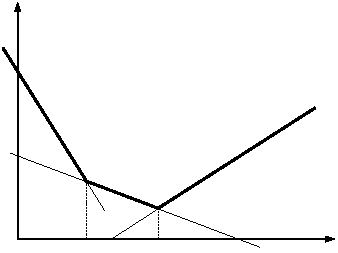
\includegraphics{part_1/chapter_6/figures/Figure2.pdf}};
	\end{tikzpicture}
	\caption{Representation of the recession cone of a polyhedral set} \label{p1c6:fig:recession_cone}	
\end{figure}

Figure \ref{p1c6:fig:recession_cone} illustrates the concept of recession cones. Notice that it is purposely placed in several places to illustrate the independence of the point $\overline{x} \in P$.

Finally, the recession cone for a standard form polyhedral set $P = \braces{x \in \reals^n : Ax = b, x \geq 0}$ is given by 
%
\begin{equation*}
	{\bf recc}(P) = \braces{d \in \reals^n : Ad = 0, d \geq 0}.	
\end{equation*} 


\subsection{Unbounded problems}

To identify unboundedness in linear programming problems, we must check for the existence of \emph{extreme rays}. Extreme rays are analogous to extreme points, but defined with a ``loose'' degree of freedom. Definition \ref{p1c6:def:extreme_ray} provides a technical definition of extreme rays.

\begin{definition}[Extreme ray] \label{p1c6:def:extreme_ray}
	Let $C \subset \reals^n$ be a nonempty polyhedral cone. A nonzero $x \in C$ is an extreme ray if there are $n-1$ linearly independent active constraints at $x$.
\end{definition} 

Notice that we are interested in extreme rays of the recession cone ${\bf recc} (P)$ of the polyhedral set $P$. However, it is typical to say that they are extreme rays of $P$. Figure \ref{p1c6:fig:extreme_rays} illustrates the concept of extreme rays in polyhedral cones.

\begin{figure}[h]
	\begin{tikzpicture}
		\node (pic) at (0,0) {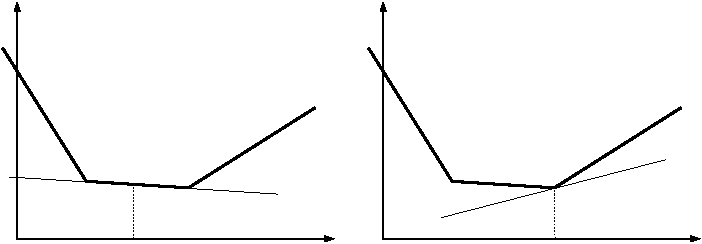
\includegraphics{part_1/chapter_6/figures/Figure3.pdf}};
		\node (x1) at (2,-2) {$x_1$};
		\node (x2) at (2,-1) {$x_2$};
		\node[right] (x3) at (-2,2) {$x_3$};
		\node (a1) at (-0.3,0.8) {$a_1$};
		\node (a2) at (1.1,-0.4) {$a_2$};
		\node[left] (d1) at (-1,0.1) {$d_1$};
		\node(d2) at (-0.4,-0.2) {$d_2$};
		\node(d3) at (0,-0.75) {$d_3$};								
	\end{tikzpicture}
	\caption{A polyhedral cone formed by the intersection of three half-spaces (the normal vector $a_3$ is perpendicular to the plane of the picture and cannot be seen). Directions $d_1$, $d_2$, and $d_3$ represent extreme rays.} \label{p1c6:fig:extreme_rays}	
\end{figure}

Notice that, just like extreme points, the number of extreme rays is finite by definition. In fact, we say that two extreme rays are equivalent if they are positive multiples corresponding to the same $n-1$ linearly independent active constraints.


The existence of extreme rays can be used to verify unboundedness in linear programming problems. The mere existence of extreme rays does not suffice since unboundedness is a consequence of the extreme ray being a direction of improvement for the objective function. To demonstrate this, let us first describe unboundedness in polyhedral cones, which we can then use to show the unboundedness in polyhedral sets.

\begin{theorem}[Unboundedness in polyhedral cones]\label{p1c6:thm:unb_cones}
	Let $P : \mini\braces{c^\top x : x \in C}$, with $C = \braces{a_i^\top x \geq 0, i = 1,\dots,m}$. The optimal value is equal to $-\infty$ if and only if some extreme ray $d \in C$ satisfies $c^\top d < 0$.
\end{theorem}

\begin{proof}
	If $c^\top d < 0$, then $P$ is unbounded, since $c^\top x \rightarrow -\infty$ along $d$. Also, there exists some $x \in C$ for which $c^\top x < 0$ can be scaled to -1.
	
	Let $P = \braces{x \in \reals^n : a_i^\top x \geq 0, i =1,\dots,m , c^\top x = -1}$. Since $0 \in C$, $P$ has at least one extreme point $\braces{a_i}_{i=1}^m$ and thus span $\reals^n$ (cf. Theorem \ref{p1c3:thm:exist_extreme_point}). Let $d$ be one of those. As we have $n$ linearly-independent active constraints at $d$, $n-1$ of the constraints $\braces{a_i^\top x \geq 0}_{i =1}^m$ must be active (plus $c^\top x = -1$), and thus $d$ is an extreme ray.
\end{proof}

We can now expand the result to general polyhedral sets.

\begin{theorem}[Unboundedness in polyhedral sets]\label{p1c6:thm:unb_polyhedra} 
	Let $P : \mini\braces{c^\top x : x \in X}$ with $X = \braces{x \in \reals^n : Ax \geq b}$ and assume that the feasible set has at least one extreme point. Then, the optimal value is $-\infty$ if and only if $c^\top d < 0$.  	
\end{theorem}

\begin{proof}
	As before, if $c^\top d < 0$, then $P$ is unbounded, since $c^\top x \rightarrow -\infty$ along $d$. Now, let 
	$D : \maxi \braces{p^\top b : p^\top A = c^\top, p \ge 0}$ be the dual of $P$. Recall that, if $P$ is unbounded, then $D$ is infeasible, and so must be $D^0 : \maxi \braces{p^\top 0 : p^\top A = c^\top, p \ge 0}$. This implies that the primal $P^0 : \mini \braces{c^\top x : Ax \geq 0}$ is unbounded (as 0 is feasible).
			
	The existence of at least one extreme point for $P$ implies that the rows $\braces{a_i}_{i=1,\dots,m}$ of $A$ span $\reals^n$ and  ${\bf recc}(X) \hspace{-3pt} =  \hspace{-3pt}\braces{x \in \reals^n : Ax \geq 0}$ is pointed. Thus, by Theorem \ref{p1c6:thm:unb_cones} there exists $d$ such that $c^\top d < 0$. \qedhere
\end{proof}

We now focus on how this can be utilised in the context of the simplex method. It turns out that once unboundedness is identified in the simplex method, one can extract the extreme ray causing the said unboundedness. In fact, most professional-grade solvers are capable of returning extreme (or unbounded) rays, which is helpful in the process of understanding the causes for unboundedness in the model. We will also see in the next chapter that these extreme rays are also used in the context of specialised solution methods.

To see that is possible, let $P : \mini\braces{c^\top x : x \in X}$ with $X = \braces{x \in \reals^n : Ax = b, x \geq 0}$ and assume that, for a given basis $B$, we conclude that the optimal value is $-\infty$, that is, the problem is unbounded. In the context of the simplex method, this implies that we found a nonbasic variable $x_j$ for which the reduced cost $\overline{c}_j < 0$ and the $j^\text{th}$ column of $B^{-1}A_j$ has no positive coefficient. Nevertheless, we can still form the feasible direction $d= [d_B ~ d_N]$ as before, with
%
\begin{equation*}
	d_B = -B^{-1}A_j \text{ and } 
	d_N = \begin{cases}
 		d_j = 1 \\
 		d_i = 0, \forall i \in I_N \setminus \braces{j}.
 	\end{cases}
\end{equation*}
%
This direction $d$ is precisely an extreme ray for $P$. To see that, first, notice that $Ad = 0$ and $d \geq 0$, thus	$d \in {\bf recc}(X)$. Moreover, there are $n-1$ active constraints at $d$: $m$ in $Ad = 0$ and $n-m-1$ in $d_i = 0$ for $i \in I_N \setminus \braces{j}$. The last thing to notice is that $\overline{c}_j = c^\top d < 0$, which shows the unboundedness in the direction $d$. 

 

\subsection{Farkas' lemma}

We now focus on the idea of generating certificates of infeasibility for linear programming problems. That is, we show that if a problem $P$ is infeasible, then there is a structure that can be identified to certify the infeasibility. To see how this works, consider the two polyhedral sets
%
\begin{align*}
	&X = \braces{x \in \reals^n : Ax = b,  x \geq 0} \text{ and } \\ 
	&Y = \braces{p \in \reals^m : p^\top A x \geq 0, p^\top b < 0}.
\end{align*}
%
If there exists any $p \in Y$, then there is no $x \in X$ for which $p^\top Ax = p^\top b$, (and in turn $Ax = b$), holds. Thus, $X$ must be empty. Notice that this can be used to infer that a problem $P$ with a feasibility set represented by $X$ prior to solving $P$ itself, by means of solving the \emph{feasibility problem} of finding a vector $p \in Y$. 

We now pose this relationship more formally via a result generally known as the Farkas' lemma.

\begin{theorem}[Farkas' lemma] \label{p1c6:thm:farkas}
	Let $A$ be a $m \times n$ matrix and $b \in \reals^m$. Then, exactly one of the following statements hold
	\begin{enumerate}
		\item[(1)] There exists some $x \geq 0$ such that $Ax = b$;
		\item[(2)] there exists some vector $p$ such that $p^\top A \geq 0$, $p^\top b < 0$. 
	\end{enumerate}
\end{theorem}

\begin{proof}
	Assume that (1) is satisfied. If $p^\top A \geq 0$, then $p^\top b =$ $p^\top Ax \geq 0$, which violates (2).
	
	Now, consider the primal-dual pair $P : \mini\braces{0^\top x : Ax = b, x \geq 0}$ and $D : \maxi\hspace{-2pt}\braces{p^\top b : p^\top A \geq 0}$. Being $P$ infeasible, $D$ must be unbounded (instead of infeasible) since $p = 0$ is feasible for $D$. Thus, $p^\top b < 0$ for some $p \neq 0$. 	
\end{proof}

The Farkas' lemma has a nice geometrical interpretation that represents the mutually exclusive relationship between the two sets. For that, notice that we can think of $b$ as being a conic combination of the columns $A_j$ of $A$, for some $x \ge 0$. If that cannot be the case, then there exists a hyperplane that separates $b$ and the cone formed by the columns of $A$, $C=\braces{y \in \reals^m : y = Ax}$. This is illustrated in Figure \ref{p1c6:fig:farkas}. Notice that the separation caused by such a hyperplane with normal vector $p$ implies that $p^\top Ax \geq 0$ and $p^\top b < 0$, i.e., $Ax$ and $b$ are on the opposite sides of the hyperplane. 

\begin{figure}[h]
	\begin{tikzpicture}
		\node (pic) at (0,0) {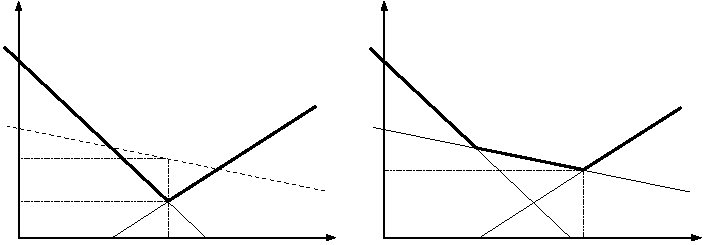
\includegraphics{part_1/chapter_6/figures/Figure4.pdf}};
		\node (A1) at (-1,0.6) {$A_1$};
		\node (A2) at (0,0.5) {$A_2$};
		\node (A3) at (1,0.4) {$A_3$};
		\node (b) at (1.6,-1) {$b$};
		\node (p) at (-1.3, -0.2) {$p$};
	\end{tikzpicture}	
	\caption{Since $b \not\in X$, $p^\top x=0$ separates them} \label{p1c6:fig:farkas}	
\end{figure}


\section{Resolution theorem*}

Lastly, we present a result that will be the foundation for our discussion in the next chapter. Specifically, we will see how we can use a presentation of the polyhedral set $P$ purely based on extreme points and extreme rays to devise solution strategies that can be more efficient for large-scale linear programming problems. 

For now, let us concentrate on this alternative representation. Basically, polyhedral sets in standard form can be represented in two manners: either by (i) a finite set of linear constraints; or (ii) by combinations of its extreme points and extreme rays.

Clearly, the first representation is far more practical than the second. That is, the second representation is an \emph{explicit} representation that would require knowing beforehand each extreme point and extreme ray forming the polyhedral set. Notice that the first representation, which we have relied on so far, has extreme points and extreme rays only implicitly represented. However, we will see that this explicit representation has an important application in the devising of alternative solution methods for large-scale linear programming problems. This fundamental result is stated in Theorem \ref{p1c6:thm:resolution_theorem}. 

\begin{theorem}[Resolution theorem]\label{p1c6:thm:resolution_theorem}
	Let $P = \braces{x \in \reals^n : Ax \geq b}$ be a nonempty polyhedral set with at least one extreme point. Let $\braces{x_i}_{i=1}^k$ be the set with all extreme points, and $\braces{w}_{j=1}^r$ be the set of all extreme rays of $P$. Then $P = Q$, where 
	\begin{equation*}
		Q = \braces{\sum_{i=1}^k \lambda_i x^i + \sum_{j=1}^r \theta_jw^j : \lambda_i \geq 0, \ \theta_j \geq 0, \ \sum_{i=1}^k \lambda_i =1}.
	\end{equation*}
\end{theorem}

%TODO: Chp6: Include proof for the resolution theorem

Theorem \ref{p1c6:thm:resolution_theorem} has an important consequence, as it states that bounded polyhedra, i.e., polyhedral sets that have no extreme rays, can be represented by the convex hull of its extreme points. For now, let us look at an example that illustrates the concept.

Consider the polyhedral set $P$ given by
%
\begin{equation*}
	P = \braces{x_1 - x_2 \geq -2; x_1 + x_2 \geq 1, x_1,x_2 \geq 0}.
\end{equation*}
%
The recession cone $C = {\bf recc}(P)$ is described by $d_1 - d_2 \geq 0$, $d_1 + d_2 \geq 0$ (from $Ad =0$), and $d_1, d_2 \geq 0$, which can be simplified as 
%
\begin{equation*}
	C = \braces{(d_1, d_2) \in \reals^2 : 0 \leq d_2 \leq d_1}.
\end{equation*}
%
We can then conclude that the two vectors $w^1 = (1,1)$ and $w_2 = (1,0)$ are extreme rays of $P$. Moreover, $P$ has three extreme points: $x_1 = (0,2)$, $x_2 = (0,1)$, and $x_3 = (1,0)$.

Figure \ref{p1c6:fig:resolution_example} illustrates what is stated in Theorem \ref{p1c6:thm:resolution_theorem}. For example,  a representation for the point $y = (2,2) \in P$ is given by
%
\begin{equation*}
	y = \begin{bmatrix} 2 \\ 2
		\end{bmatrix}= \begin{bmatrix} 0 \\ 1
		\end{bmatrix} + \begin{bmatrix} 1 \\ 1
		\end{bmatrix} + \begin{bmatrix} 1 \\ 0
		\end{bmatrix}, 	
\end{equation*}
%
that is, $y = x^2 + w^1 + w^2$. Notice however, that $y$ could also be represented as 
%
\begin{equation*}
	y = \begin{bmatrix} 2 \\ 2
		\end{bmatrix}= \frac{1}{2}\begin{bmatrix} 0 \\ 1
		\end{bmatrix} + \frac{1}{2}\begin{bmatrix} 1 \\ 0
		\end{bmatrix} + \frac{3}{2}\begin{bmatrix} 1 \\ 1
		\end{bmatrix}, 	
\end{equation*}
%
with then $y = = \frac{1}{2}x^2 + \frac{1}{2}x^3 + \frac{3}{2}w^1$. Notice that this imply that the representation of each point is not unique.

\begin{figure}[h]
	\includegraphics{part_1/chapter_6/figures/Figure5.pdf}
	\caption{Example showing that every point of $P = \braces{x_1 - x_2 \geq -2; x_1 + x_2 \geq 1, x_1,x_2 \geq 0}$ can be represented as a convex combination of its extreme point and a linear combination of its extreme rays} \label{p1c6:fig:resolution_example}
\end{figure}

\pagebreak	

\section{Exercises}

\subsection*{Exercise 6.1: Sensitivity analysis in the RHS}
Consider the following linear programming problem and its optimal tableau below:

\begin{align*}
	\mini & -2x_1 - x_2 + x_3 \\
	\st   & x_1 + 2x_2 + x_3 \le 8 \\
		  & -x_1 + x_2 - 2x_3 \le 4 \\
		  & 3x_1 + x_2 \le 10 \\
		  & x_1, x_2, x_3 \ge 0.	 
\end{align*}

\begin{center}
	\begin{tabular}{c|cccccc|c}
		        & $x_1$ & $x_2$ & $x_3$ & $x_4$ & $x_5$ & $x_6$ & RHS \\
		\hline
		    $z$ &   0   &   0   &   1.2 &   0.2 &   0   &   0.6 & -7.6 \\
		\hline
		  $x_1$ &   1   &   0   &  -0.2 &  -0.2 &   0   &   0.4 &  2.4  \\
		  $x_2$ &   0   &   1   &   0.6 &   0.6 &   0   &  -0.2 &  2.8  \\
		  $x_5$ &   0   &   0   &  -2.8 &  -0.8 &   1   &   0.6 &  3.6  \\
	\end{tabular}	
\end{center}


\begin{itemize}
	\item [(a)] If you were to choose between increasing in 1 unit the right-hand side of any constraints, which one would you choose, and why? What is the effect of the increase on the optimal cost?
	\item [(b)] Perform a sensitivity analysis on the model to discover what is the range of alteration in the RHS in which the same effect calculated in item (a) can be expected. \emph{HINT}: JuMP (from version 0.21.6) includes the function ``lp\_sensitivity\_report()'' that you can use to help performing the analysis.
\end{itemize}


\subsection*{Exercise 6.2: Extreme points and extreme rays}
\input{part_1/chapter_6/exercises/E62-extremerays}

\subsection*{Exercise 6.3: From Farkas' lemma to duality}
Use the Farkas' lemma to prove the duality theorem for a linear programming problem involving constraints of the form $a'_ix = b_i, a'_ix \geq b_i$, and nonegativity constraints for some of the variables $x_j$. \emph{Hint}: Start by deriving the form of the set of feasible directions at an optimal solution.


\subsection*{Exercise 6.4: Adding a constraint}
Consider the linear programming problem below with optimal basis $[x_1, x_2, x_5, x_6]$ and dual variables $p_1, \dots, p_4$.

\begin{align*}
	\maxi & 2x_1 + x_2 \\
	\st   & 2x_1 + 2x_2 \le 9 \quad (p_1) \\
	      & 2x_1 - x_2 \le 3 \quad (p_2) \\
	      & x_1 \le 3 \quad (p_3) \\
	      & x_2 \le 4 \quad (p_4) \\
	      & x_1, x_2 \ge 0.
\end{align*}

\begin{itemize}
	\item[(a)] Find the primal and dual optimal solutions. \emph{HINT}: You can use complementary slackness, once having the primal optimum, to find the dual optimal solution.
	\item[(b)] Suppose we add a new constraint $6x_1 - x_2 \leq 6$, classify the primal and dual former optimal points stating if they: (i) remain optimal; (ii) remain feasible but not optimal; or (iii) become infeasible.
	\item[(c)] Consider the new problem from item (b) and find the new dual optimal point through one dual simplex iteration. After that, find the primal optimum.
\end{itemize}







